\documentclass[12pt]{article}

\usepackage{graphicx,amsmath}

\title{CSCI 5454 Final Project: AVL Tree}
\author{Robert Werthman}
\date{}

\begin{document}

\maketitle

\newpage
\tableofcontents

\newpage
\addcontentsline{toc}{section}{Introduction}
\section*{Introduction}

\addcontentsline{toc}{subsection}{What is an AVL Tree?}
\subsection*{What is an AVL Tree?}

An AVL tree is a binary search tree that is ``self-balancing''.  This means
after each operation, like an insertion or deletion, on the tree the heights of 
each node's children differ by at most 1.  The height of a node is the number of
nodes in the longest path from it to a leaf node.  A leaf node
always has a height of 0. Its parent node, if the leaf
node was the parent's only child, would have a height of 1.  An AVL tree is
``self-balancing'' because after each tree operation the heights and balance of
the nodes are readjusted by the tree \cite{wiki:avl}.

\addcontentsline{toc}{subsection}{What problems does it solve?}
\subsection*{What problems does it solve?}
AVL trees, like binary trees, are used for storing and retrieving
information.  Their advantage is that they can perform these operations faster
than if the information was stored in an array.  As will be shown later in this
paper, storing and retrieving takes log $n$ time for an AVL tree
while performing the same operations on an array could take up to $n$ time.

\addcontentsline{toc}{subsection}{Where is it used?}
\subsection*{Where is it used?}
Red-black trees, another kind of self-balancing binary search tree, are
typically used instead of AVL trees in real world applications
\cite{wiki:red-black}.
Red-black trees can be found in the C++ Standard Library (std) as the underlying data structure
for the std::map and std::set containers and it is reasonable to think that AVL
trees could be used instead.

\addcontentsline{toc}{section}{Mathemetical Analysis of Correctness, Runtime, and Space}
\section*{Mathemetical Analysis of Correctness, Runtime, and Space}

\addcontentsline{toc}{subsection}{Correctness}
\subsection*{Correctness}
The correctness of the AVL tree relies on maintaining two invariants
\begin{enumerate}
  \item The height of a node is the number of nodes in the longest path from it
  to a leaf node.
  \item The heights of each node's children differ by at most 1.  This is
  demonstrated by the equation $|x-y| \le 1$ where x is the height of the left
  child node and y is the height of the right child node.
\addcontentsline{toc}{subsubsection}{Basecase}
\subsubsection*{Basecase}
\end{enumerate}
\begin{figure}[h]
\caption{An AVL tree with a single node}
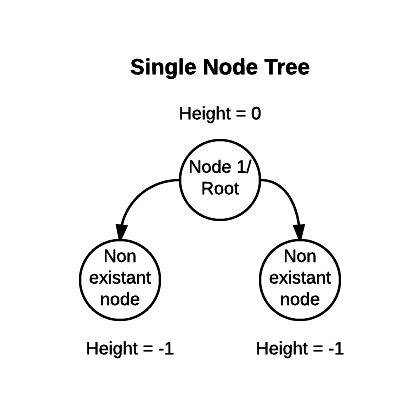
\includegraphics{single_node_tree.png}
\centering
\end{figure}
\noindent
We will use the insertion operation to show these invariants are maintained. 
We first start with a single, leaf node in a tree as the base case as shown in
Figure 1.  First, we let the height of any non existent node be equal to -1.
This means a single node in a tree has two non existent children nodes each
with a height of -1.  To find the height of the single node in the tree we take the max of the
heights of the children and then add 1 to it to always maintain the first
invariant.  In this case max(-1, -1) = -1 and adding 1 to this result gives a
height of 0 for the single node in the tree.  To make sure the second invariant
is maintained we use the given equation
$$
|x-y| \le 1
$$
In the case of a single, leaf node the height of the left child is
-1 and the height of the right child is -1.  Substituting these values in for
$x$ and $y$ produces the equation
\begin{align*}
|(-1)-(-1)| &= 0\\
&\le 1
\end{align*}
Since $0 \le 1$ the second invariant is maintained.
\addcontentsline{toc}{subsubsection}{Inductive Proof of the First Invariant}
\subsubsection*{Inductive Proof of the First Invariant}
Next it must be inductively shown that the two invariants hold for every AVL
tree with size greater than 1 node.  Concerning the first invariant, every time
a new node is inserted into the AVL tree, it will be a leaf node with a height
of 0 as was demonstrated in the base case.  Once an insertion takes place, the
AVL tree updates the the balances and heights of the new node and all of the
nodes above it.  This is done by recursing through 
the parent nodes, starting with the inserted node and moving upwards to the
root.  The height of each parent node is equal to the max of
the childrens' heights plus 1.  Since this update of the heights is bottom up
and takes place for every node inserted into the tree, the first invariant holds for any tree of
size greater than 1 nodes.\\
\addcontentsline{toc}{subsubsection}{Inductive Proof of the Second Invariant}
\subsubsection*{Inductive Proof of the Second Invariant}
To show the correctness of the second invariant we have to look at the possible
cases of a tree being out of balance and how those are corrected.
\begin{figure}[h]
\caption{Left and Right Tree Rotations}
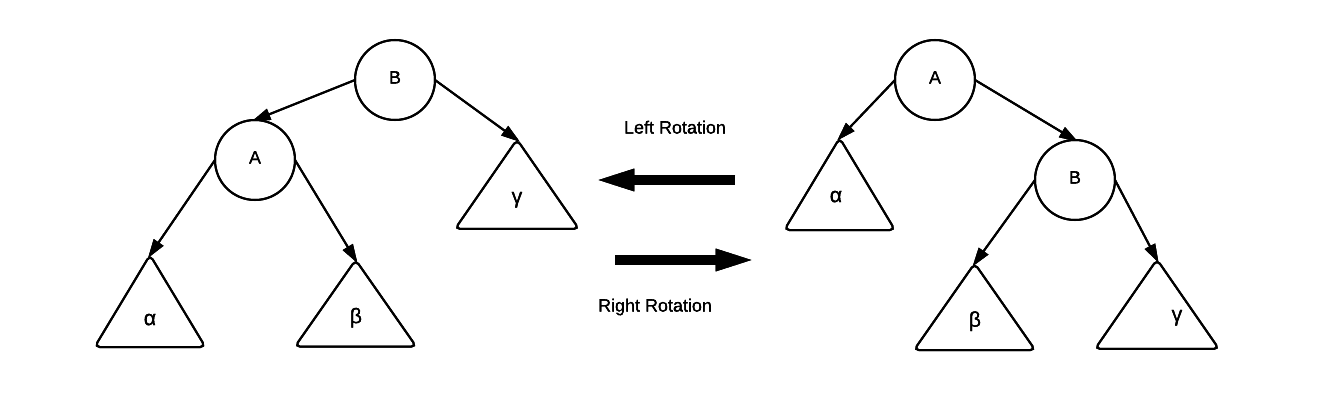
\includegraphics[width=15cm]{tree_rotations.png}
\centering
\end{figure}
\noindent
In order for an AVL tree to remain in balance, the tree has to
perform what are known as tree rotations after nodes are inserted.
\cite{wiki:avl}.
The basic two rotations can be seen in Figure 2.  During tree rotations, the
shape of a tree is modified in order to change the heights of subtrees
at a particular node.  For example, doing a right rotation of the tree in
Figure 2 ``increases'' the height of node A while ``decreasing'' the height of
node B \cite{wiki:tree-rotations}.  These can be judiciously used to rebalance
the tree and maintain the second invariant of an AVL tree.\\
\\
When a node is inserted, the first thing that the tree does is check
the balance at the inserted node and all of the nodes above to
ensure that the equation for the second invariant is maintained.  If the
balances of any of the nodes do not satsify the second invariant equation, tree
rotations must take place in order to balance the tree.  
Four cases of an unbalanced tree may occur after a node is inserted into a tree,
as shown in Figures 3-6.  These may require one or more
rotations to rebalance a tree \cite{tutorialspoint:avl}.
\begin{figure}[h]
\caption{Right Unbalanced Tree}
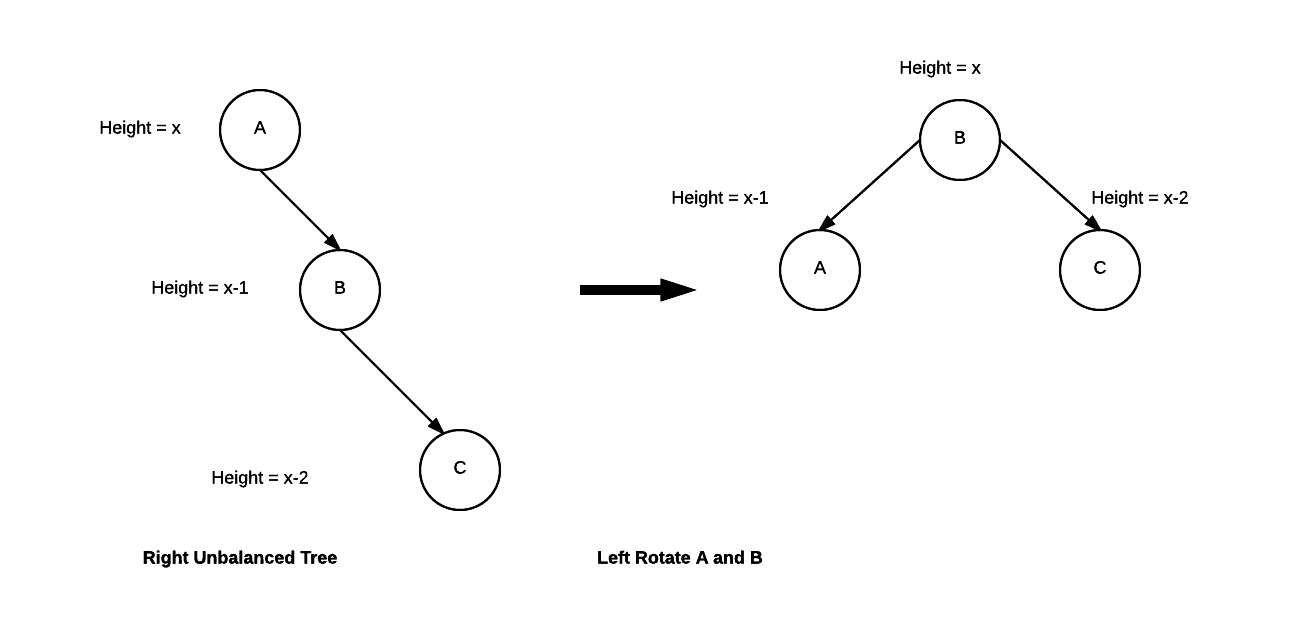
\includegraphics[width=15cm]{right_unbalanced_tree.png}
\centering
\end{figure}
\noindent
\begin{figure}[h]
\caption{Left Unbalanced Tree}
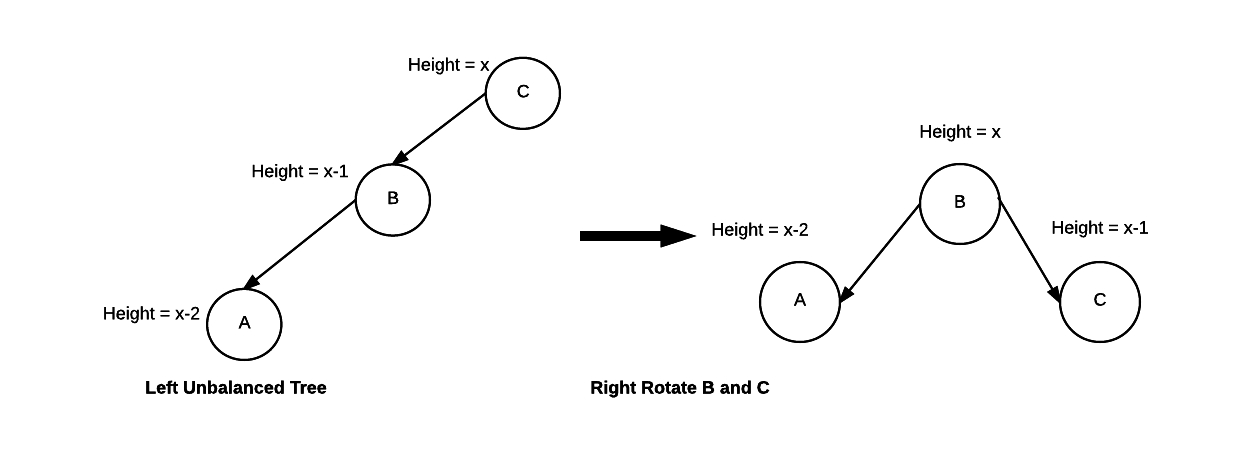
\includegraphics[width=15cm]{left_unbalanced_tree.png}
\centering
\end{figure}
\noindent
\begin{figure}[h]
\caption{Right Left Unbalanced Tree}
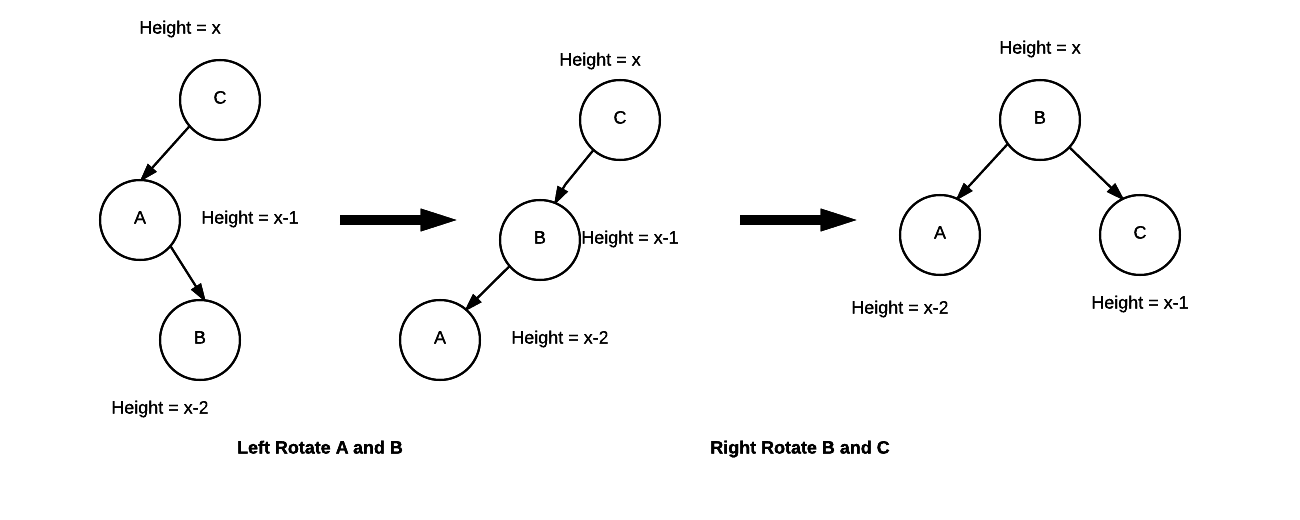
\includegraphics[width=15cm]{right_left_unbalanced_tree.png}
\centering
\end{figure}
\noindent
\begin{figure}[h]
\caption{Left Right Unbalanced Tree}
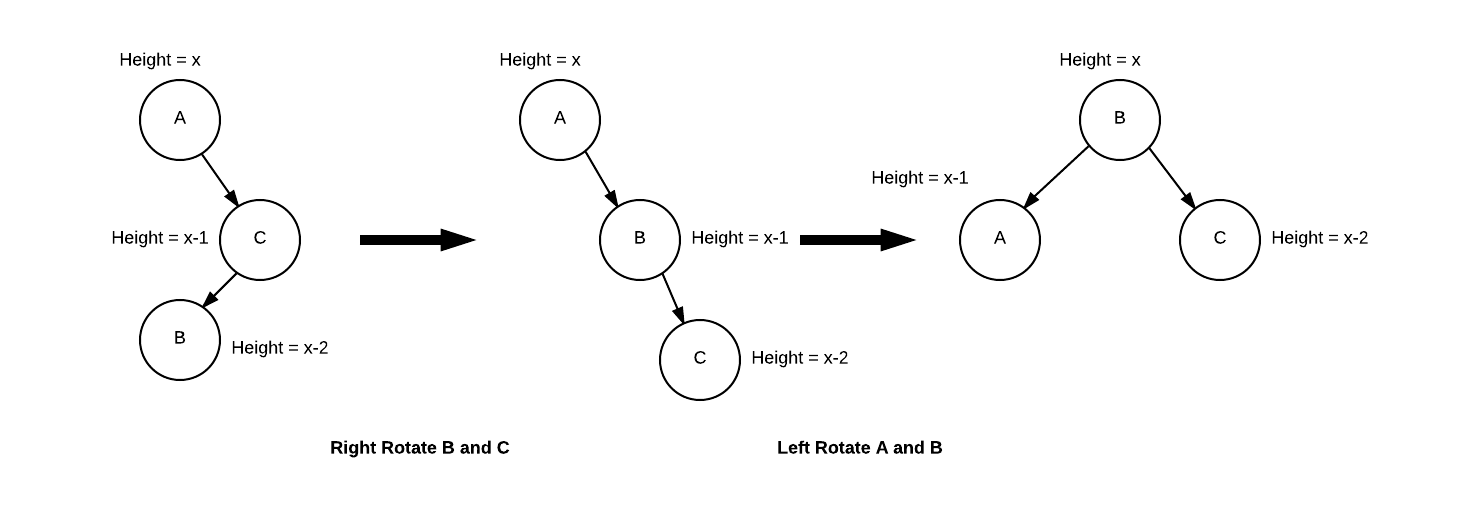
\includegraphics[width=15cm]{left_right_unbalanced_tree.png}
\centering
\end{figure}
\noindent
Once one or more rotations of the subtrees of a node take place and that node
is balanced according to the second invariant equation, the height of that node
and any of the other nodes invovled in the rotation are updated.  The
tree then recursively checks the node's parents, grandparents, etc. 
until the root of the tree is reached for correct balances, performing any 
rotations if necessary, and updating the heights as it moves upwards through
the tree.  This method of updating the balances and heights ensures that given
any number of inserted nodes, the tree with always be rebalanced and each node will
have the correct height.

\addcontentsline{toc}{subsection}{Runtime}
\subsection*{Runtime}
Since an AVL tree is a binary search tree any AVL tree operations' runtime
depends on the trees height, which is the longest path from the root node to a
leaf -- also known as its longest branch \cite{avl-runtime}.  In order to prove
the runtime any AVL tree operations is O(log n) we need to show that the height of an AVL tree
can be bounded by O(log n).\\
\\
Let the root of the AVL tree have a height of $h$.  
One child of the root will have a height of $h-1$ and the other, if we follow 
the property of an AVL tree that says the heights of the children differ by at 
most 1, will have a minimum height of $h-2$.  Let $n_h$ be the number of nodes
in the tree including the root.  Let $n_{h-1}$ be the number of nodes underneath
and including the child of the root with height $h-1$ and $n_{h-2}$ be the
number of nodes underneath and including the child with height $h-2$.  We can
construct the total size of the tree $n_h$ by using the recurrence relation
$$
n_h = n_{h-1} + n_{h-2} + 1
$$
We can bound the height of the AVL tree by unrolling the recurrence relation
with the following setps:
\begin{align}
n_h &= n_{h-1} + n_{h-2} + 1\\
n_{h-1} &= n_{h-2} + n_{h-3} + 1\\
n_h &= (n_{h-2} + n_{h-3} + 1) + n_{h-2} + 1\\
n_h &> 2n_{h-2} > 2(2n_{h-4}) > 2(2(2n_{h-6})) > \ldots > 2^{\frac{h}{2}}\\
\text{log }n_h &> \text{log }2^{\frac{h}{2}}\\
\text{log }n_h &> \frac{h}{2}\\
2\text{log }n_h &> h
\end{align}
This shows that the height $h$ of an AVL tree will always be bounded by
O(log $n$).
This means the runtime for any AVL tree operation will be bounded by O(log $n$).
\addcontentsline{toc}{subsection}{Space}
\subsection*{Space}
The space an AVL tree uses is equal the number of the nodes in the tree.  If
there are $n + 1$ nodes inserted into the tree, the space used will be $n + 1$. 
If there are $n - 1$ nodes removed from the tree, the space used will be $n-1$. 
The space is equal to $\theta(n)$.

\addcontentsline{toc}{section}{Numerical Characterization of Runtime and Space}
\section*{Numerical Characterization of Runtime and Space}

\addcontentsline{toc}{subsection}{Description of the code invloved in the Numerical Characterization}
\subsection*{Description of the code invloved in the Numerical Characterization}
To show the numerical characterization of the space and time performance of an
AVL tree, I created a randomized input generator to show the runtime and space
of the three operations that can be performed on the AVL tree: insertion,
deletion, and search.  I ran 12 iterations for each of these tree operations,
varying the number of nodes $n$ in the tree by a factor of 2.  I ran each of
these iterations 50 times each to find the average number of operations given a
value of $n$.  $n$ takes on all of the values in the set
$\{2^4,\,2^5,\ldots,2^{16}\}$ for each tree operation.
The keys for each of the nodes in the $n$ node-sized tree were randomly chosen
from the set $\{0,1,\ldots,n\}$ and then inserted into the tree to create a
tree of size $n$.\\
\\
Once the tree was generated for an iteration, I then chose a random key
from the set of keys that were already in the tree, and I either searched for
it, inserted it, or deleted it.  To keep track of the runtime when performing
these operations on the tree, I kept a global variable as a counter and
incremented it every time an atomic operation occurred.  To keep track of the space used when
performing these operations on the tree, I kept a global variable as a counter
and incremented it when a node was inserted and decremented it when a node was
removed from the tree.  These global variables were reset after each
iteration.\\
\\
Once all the iterations were complete for a specific operation, I took the $n$
for each iteration and the values of the global variables for each iteration and
graphed them as a function $f(x)$.  The values of $n$ were placed on the
x-axis and the values of the globabl variables were placed on the y-axis.  The graphs use the logarithmic
scale instead of the linear scale because the logarthmic scale more clearly
shows what $n$ and the values of the global variables are doing.
I then graphed one other line representing the function $g(x)$, which is
the function that bounds $f(x)$. $g(x)$ is then
multiplied by a constant, $c_2$, producing a separate line.
\addcontentsline{toc}{subsection}{Characterization of Runtime}
\subsection*{Characterization of Runtime}

\addcontentsline{toc}{subsubsection}{Runtime of Search}
\subsubsection*{Runtime of Search}
\begin{figure}[h]
\caption{Graph of the runtime for searching for a key in different-sized AVL
trees}
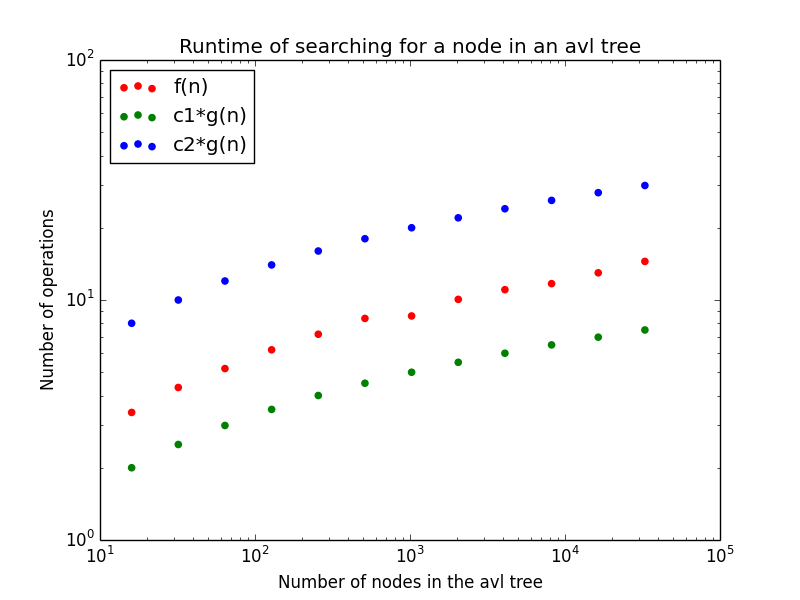
\includegraphics[width=9cm]{search_runtime.png}
\centering
\end{figure}
\noindent
Figure 7 shows the runtime for searching for a key in different-sized
avl trees.
The function that bounds the runtime of search is $g(n)= \text{log }n$ multiplied by
the constant $c_2=2$.  As can be seen in the graph, the
runtime of search is O(log $n$), with the function log $n$ bounding the
search runtime from above.  This means given an AVL tree of size $n$, it will
take O(log $n$) operations to search for key in the tree.

\addcontentsline{toc}{subsubsection}{Runtime of Insert}
\subsubsection*{Runtime of Insert}
\begin{figure}[h]
\caption{Graph of the runtime for inserting a key into different-sized AVL
trees}
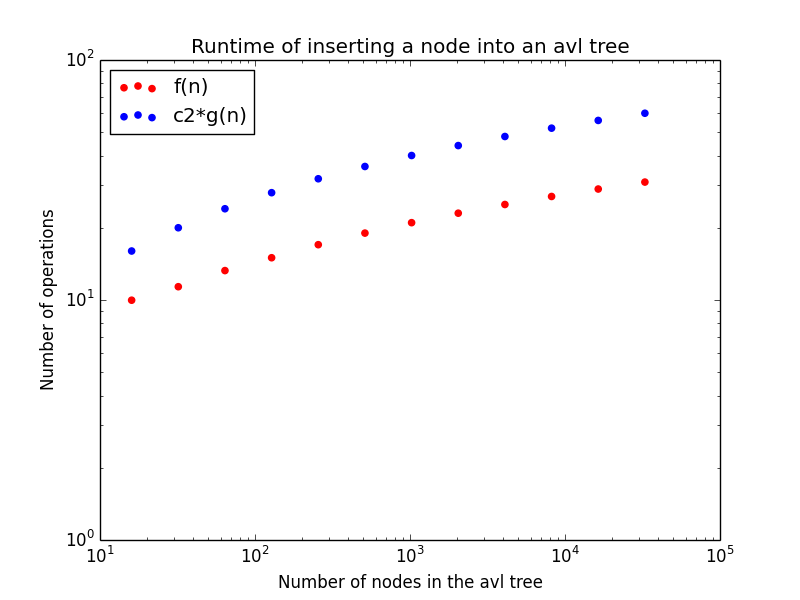
\includegraphics[width=9cm]{insert_runtime.png}
\centering
\end{figure}
\noindent
Figure 8 shows the runtime for inserting a key into different-sized AVL
trees.  The function that bounds the runtime of insert is $g(n)= \text{log }n$
multiplied by the constant $c_2=4$.  As can be seen in the graph the runtime of
insert is O(log $n$), with the function log $n$ bounding the insert runtime
from above.  This means given an AVL tree of size $n$, it will take O(log $n$)
operations to insert a key into the tree.

\addcontentsline{toc}{subsubsection}{Runtime of Delete}
\subsubsection*{Runtime of Delete}
\begin{figure}[h]
\caption{Graph of the runtime for deleting a key from different-sized AVL
trees}
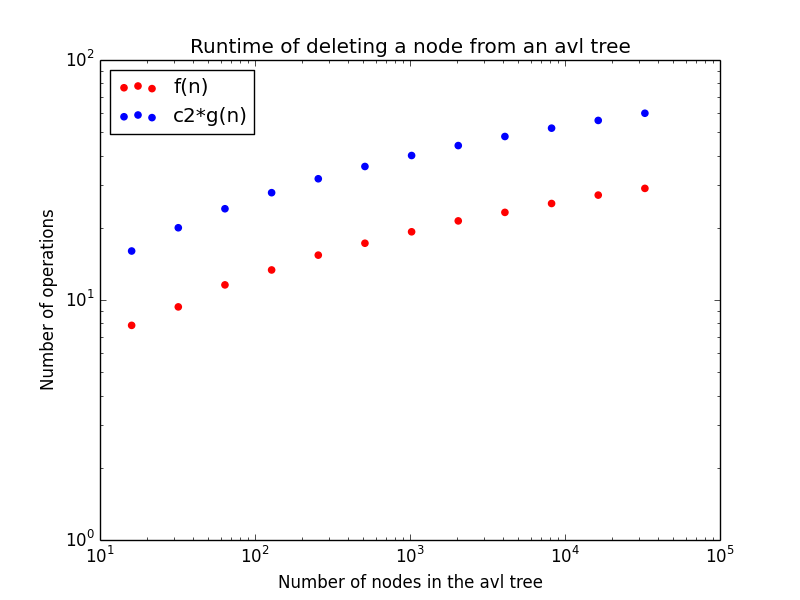
\includegraphics[width=9cm]{delete_runtime.png}
\centering
\end{figure}
\noindent
Figure 9 shows the runtime of deleting a key from different-sized AVL
trees.  The function that bounds the runtime of delete is $g(n)= \text{log }n$
multiplied by the constant $c_2=4$.  As can be seen in the graph the runtime of
delete is O(log $n$), with the function log $n$ bounding the delete runtime
from above.  This means given an AVL tree of size $n$, it will take O(log $n$)
operations to delete a key from the tree.

\addcontentsline{toc}{subsection}{Characterization of Space Usage}
\subsection*{Characterization of Space Usage}
\begin{figure}[h]
\caption{Graph of the space used by different-size AVL trees}
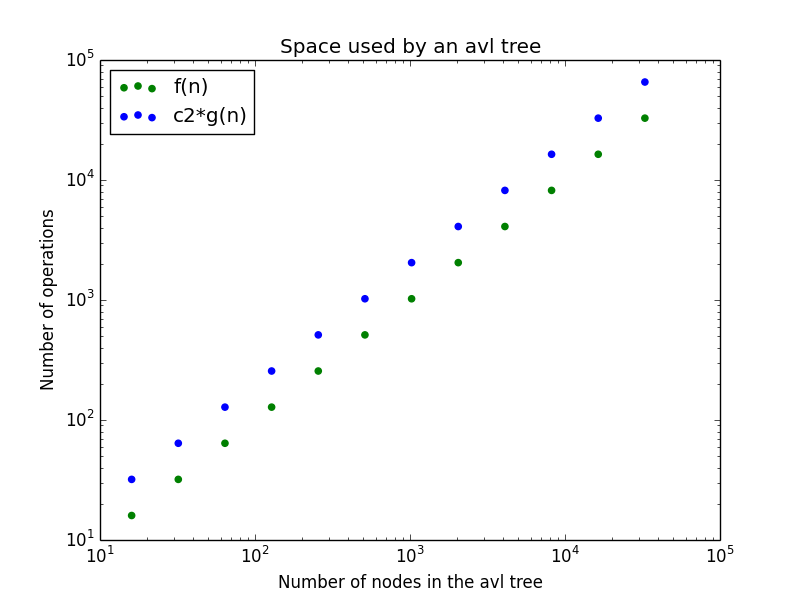
\includegraphics[width=9cm]{space_used.png}
\centering
\end{figure}
\noindent
Figure 10 shows the space used by different-size AVL trees.  The function
that bounds the space used by an AVl tree is $g(n) = n$ multiplied by the
constant $c_2 = 2$.  As can be seen in the graph the space that is used by an
AVL tree is O($n$), with the function $n$ bounding the space used from above.  This means that given
an AVL tree of size $n$, there will be exaclty $n$ nodes in the tree.  With a
tree of size $n$, if a node is inserted there will be $n+1$ nodes in the tree. 
With a tree of size $n$, if a node is deleted there will be $n-1$ nodes in the
tree.

\addcontentsline{toc}{section}{Extensions, Improvements, and Recent Work}
\section*{Extensions, Improvements, and Recent Work}
There has been work done recently to improve the time it takes to rebalance an
AVL tree.  A relaxation of AVL tree balance constraints produces a new data
structure called a weak AVL tree (wavl).  It has been shown that insert and delete take at
most ``two rotations'' in the worst case and ``O(1)'' amortized time.  This is
fewer rotations than the number of rotations a regular AVL tree and red-black
tree need to perform to rebalance \cite{avl-improvments}.\\
\\
A relaxed version of an AVL tree was also proposed to be used in a 
``concurrent tree algorithm'' to improve thread throughput.  In this case, an
AVL tree acts like a map object with operations like ``get, put, remove.'' 
An AVL tree is relaxed because balancing of the tree is delayed until after the 
map operations take place on the tree \cite{avl-concurrent}.

\newpage
\addcontentsline{toc}{section}{References}

\bibliographystyle{unsrt}
\bibliography{sources}


\end{document}